\documentclass{book}
\usepackage[a4paper,top=2.5cm,bottom=2.5cm,left=2.5cm,right=2.5cm]{geometry}
\usepackage{makeidx}
\usepackage{natbib}
\usepackage{graphicx}
\usepackage{multicol}
\usepackage{float}
\usepackage{listings}
\usepackage{color}
\usepackage{ifthen}
\usepackage[table]{xcolor}
\usepackage{textcomp}
\usepackage{alltt}
\usepackage{ifpdf}
\ifpdf
\usepackage[pdftex,
            pagebackref=true,
            colorlinks=true,
            linkcolor=blue,
            unicode
           ]{hyperref}
\else
\usepackage[ps2pdf,
            pagebackref=true,
            colorlinks=true,
            linkcolor=blue,
            unicode
           ]{hyperref}
\usepackage{pspicture}
\fi
\usepackage[utf8]{inputenc}
\usepackage{mathptmx}
\usepackage[scaled=.90]{helvet}
\usepackage{courier}
\usepackage{sectsty}
\usepackage{amssymb}
\usepackage[titles]{tocloft}
\usepackage{doxygen}
\lstset{language=C++,inputencoding=utf8,basicstyle=\footnotesize,breaklines=true,breakatwhitespace=true,tabsize=4,numbers=left }
\makeindex
\setcounter{tocdepth}{3}
\renewcommand{\footrulewidth}{0.4pt}
\renewcommand{\familydefault}{\sfdefault}
\hfuzz=15pt
\setlength{\emergencystretch}{15pt}
\hbadness=750
\tolerance=750
\begin{document}
\hypersetup{pageanchor=false,citecolor=blue}
\begin{titlepage}
\vspace*{7cm}
\begin{center}
{\Large Database\-Application }\\
\vspace*{1cm}
{\large Generated by Doxygen 1.8.3.1}\\
\vspace*{0.5cm}
{\small Wed Feb 27 2013 18:52:54}\\
\end{center}
\end{titlepage}
\clearemptydoublepage
\pagenumbering{roman}
\tableofcontents
\clearemptydoublepage
\pagenumbering{arabic}
\hypersetup{pageanchor=true,citecolor=blue}
\chapter{Hierarchical Index}
\section{Class Hierarchy}
This inheritance list is sorted roughly, but not completely, alphabetically\-:\begin{DoxyCompactList}
\item \contentsline{section}{Database}{\pageref{class_database}}{}
\item exception\begin{DoxyCompactList}
\item \contentsline{section}{Column\-Does\-Not\-Exist\-Error}{\pageref{class_column_does_not_exist_error}}{}
\item \contentsline{section}{Invalid\-Operation\-Error}{\pageref{class_invalid_operation_error}}{}
\begin{DoxyCompactList}
\item \contentsline{section}{Key\-Conflict\-Error}{\pageref{class_key_conflict_error}}{}
\end{DoxyCompactList}
\item \contentsline{section}{Invalid\-Type\-Error}{\pageref{class_invalid_type_error}}{}
\item \contentsline{section}{I\-O\-Error}{\pageref{class_i_o_error}}{}
\item \contentsline{section}{Query\-Syntax\-Error}{\pageref{class_query_syntax_error}}{}
\item \contentsline{section}{Row\-Does\-Not\-Exist\-Error}{\pageref{class_row_does_not_exist_error}}{}
\item \contentsline{section}{Table\-Does\-Not\-Exist\-Error}{\pageref{class_table_does_not_exist_error}}{}
\end{DoxyCompactList}
\item \contentsline{section}{Record}{\pageref{class_record}}{}
\item \contentsline{section}{Table}{\pageref{class_table}}{}
\item \contentsline{section}{Type\-Is\-Valid$<$ T $>$}{\pageref{struct_type_is_valid}}{}
\item \contentsline{section}{Type\-Is\-Valid$<$ const char $\ast$ $>$}{\pageref{struct_type_is_valid_3_01const_01char_01_5_01_4}}{}
\item \contentsline{section}{Type\-Is\-Valid$<$ double $>$}{\pageref{struct_type_is_valid_3_01double_01_4}}{}
\item \contentsline{section}{Type\-Is\-Valid$<$ float $>$}{\pageref{struct_type_is_valid_3_01float_01_4}}{}
\item \contentsline{section}{Type\-Is\-Valid$<$ int $>$}{\pageref{struct_type_is_valid_3_01int_01_4}}{}
\item \contentsline{section}{Type\-Is\-Valid$<$ string $>$}{\pageref{struct_type_is_valid_3_01string_01_4}}{}
\end{DoxyCompactList}

\chapter{Class Index}
\section{Class List}
Here are the classes, structs, unions and interfaces with brief descriptions\-:\begin{DoxyCompactList}
\item\contentsline{section}{\hyperlink{class_column_does_not_exist_error}{Column\-Does\-Not\-Exist\-Error} }{\pageref{class_column_does_not_exist_error}}{}
\item\contentsline{section}{\hyperlink{class_database}{Database} }{\pageref{class_database}}{}
\item\contentsline{section}{\hyperlink{class_invalid_operation_error}{Invalid\-Operation\-Error} }{\pageref{class_invalid_operation_error}}{}
\item\contentsline{section}{\hyperlink{class_invalid_type_error}{Invalid\-Type\-Error} }{\pageref{class_invalid_type_error}}{}
\item\contentsline{section}{\hyperlink{class_i_o_error}{I\-O\-Error} }{\pageref{class_i_o_error}}{}
\item\contentsline{section}{\hyperlink{class_key_conflict_error}{Key\-Conflict\-Error} }{\pageref{class_key_conflict_error}}{}
\item\contentsline{section}{\hyperlink{class_query_syntax_error}{Query\-Syntax\-Error} }{\pageref{class_query_syntax_error}}{}
\item\contentsline{section}{\hyperlink{class_record}{Record} }{\pageref{class_record}}{}
\item\contentsline{section}{\hyperlink{class_row_does_not_exist_error}{Row\-Does\-Not\-Exist\-Error} }{\pageref{class_row_does_not_exist_error}}{}
\item\contentsline{section}{\hyperlink{class_table}{Table} }{\pageref{class_table}}{}
\item\contentsline{section}{\hyperlink{class_table_does_not_exist_error}{Table\-Does\-Not\-Exist\-Error} }{\pageref{class_table_does_not_exist_error}}{}
\item\contentsline{section}{\hyperlink{struct_type_is_valid}{Type\-Is\-Valid$<$ T $>$} }{\pageref{struct_type_is_valid}}{}
\item\contentsline{section}{\hyperlink{struct_type_is_valid_3_01const_01char_01_5_01_4}{Type\-Is\-Valid$<$ const char $\ast$ $>$} }{\pageref{struct_type_is_valid_3_01const_01char_01_5_01_4}}{}
\item\contentsline{section}{\hyperlink{struct_type_is_valid_3_01double_01_4}{Type\-Is\-Valid$<$ double $>$} }{\pageref{struct_type_is_valid_3_01double_01_4}}{}
\item\contentsline{section}{\hyperlink{struct_type_is_valid_3_01float_01_4}{Type\-Is\-Valid$<$ float $>$} }{\pageref{struct_type_is_valid_3_01float_01_4}}{}
\item\contentsline{section}{\hyperlink{struct_type_is_valid_3_01int_01_4}{Type\-Is\-Valid$<$ int $>$} }{\pageref{struct_type_is_valid_3_01int_01_4}}{}
\item\contentsline{section}{\hyperlink{struct_type_is_valid_3_01string_01_4}{Type\-Is\-Valid$<$ string $>$} }{\pageref{struct_type_is_valid_3_01string_01_4}}{}
\end{DoxyCompactList}

\chapter{File Index}
\section{File List}
Here is a list of all documented files with brief descriptions\-:\begin{DoxyCompactList}
\item\contentsline{section}{{\bfseries database.\-h} }{\pageref{database_8h}}{}
\item\contentsline{section}{\hyperlink{exception_8h}{exception.\-h} }{\pageref{exception_8h}}{}
\item\contentsline{section}{{\bfseries record.\-h} }{\pageref{record_8h}}{}
\item\contentsline{section}{{\bfseries table.\-h} }{\pageref{table_8h}}{}
\end{DoxyCompactList}

\chapter{Class Documentation}
\hypertarget{class_column_does_not_exist_error}{\section{Column\-Does\-Not\-Exist\-Error Class Reference}
\label{class_column_does_not_exist_error}\index{Column\-Does\-Not\-Exist\-Error@{Column\-Does\-Not\-Exist\-Error}}
}
Inheritance diagram for Column\-Does\-Not\-Exist\-Error\-:\begin{figure}[H]
\begin{center}
\leavevmode
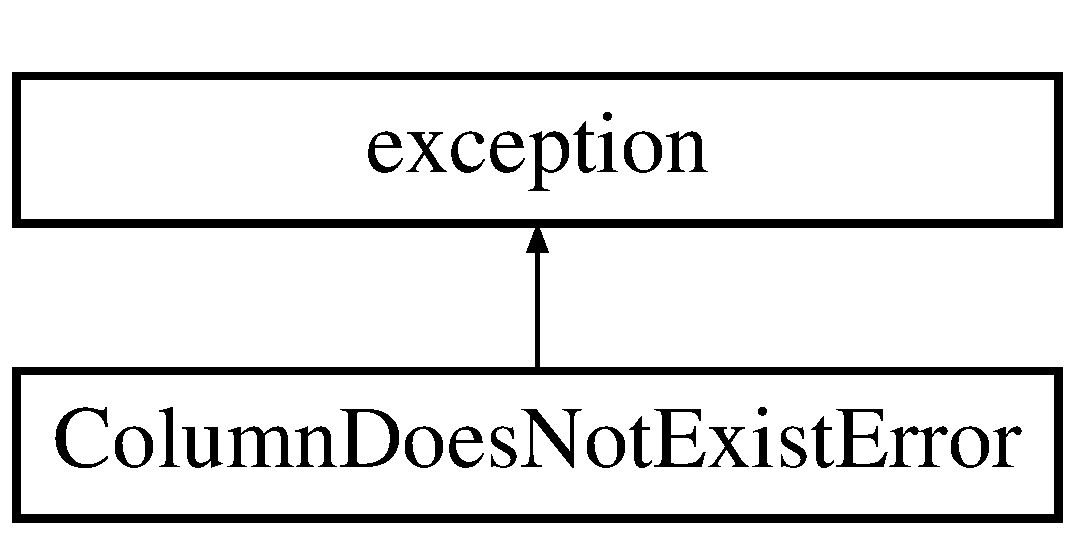
\includegraphics[height=2.000000cm]{class_column_does_not_exist_error}
\end{center}
\end{figure}
\subsection*{Public Member Functions}
\begin{DoxyCompactItemize}
\item 
\hypertarget{class_column_does_not_exist_error_ae4d5e02900c814ec4d64f78559911357}{{\bfseries Column\-Does\-Not\-Exist\-Error} (const string \&what)}\label{class_column_does_not_exist_error_ae4d5e02900c814ec4d64f78559911357}

\end{DoxyCompactItemize}


The documentation for this class was generated from the following file\-:\begin{DoxyCompactItemize}
\item 
\hyperlink{exception_8h}{exception.\-h}\end{DoxyCompactItemize}

\hypertarget{class_database}{\section{Database Class Reference}
\label{class_database}\index{Database@{Database}}
}


{\ttfamily \#include $<$database.\-h$>$}

\subsection*{Public Member Functions}
\begin{DoxyCompactItemize}
\item 
\hyperlink{class_database_a4703c80e6969d33565ea340f768fdadf}{Database} ()
\item 
void \hyperlink{class_database_a1f7550b57bc33787114c40078a38e36d}{add\-\_\-table} (string name, \hyperlink{class_table}{Table} $\ast$\hyperlink{class_database_a73027c54c1f7907d48aa31a1196c4238}{table})
\item 
void \hyperlink{class_database_abe4f1ffd1e94eddfeff6634b25a8d905}{drop\-\_\-table} (string name)
\item 
vector$<$ string $>$ \hyperlink{class_database_a9706507bd920dcea216553b08e995eb7}{table\-\_\-names} ()
\item 
\hyperlink{class_table}{Table} $\ast$ \hyperlink{class_database_a73027c54c1f7907d48aa31a1196c4238}{table} (string table\-\_\-name)
\item 
\hyperlink{class_table}{Table} $\ast$ \hyperlink{class_database_a15b71527a4147465453e83c9f0cb0852}{table\-\_\-if\-\_\-exists} (string table\-\_\-name)
\item 
\hyperlink{class_table}{Table} $\ast$ \hyperlink{class_database_a0520f606f68e207ca972e1c84b625805}{query} (string select, string from, string where)
\item 
void \hyperlink{class_database_a12693f5c16b9e8c42cbaee651aa91383}{delete\-\_\-from} (string from, string where)
\item 
void \hyperlink{class_database_a16075d5f6abe6faaa9b33fdeb224fb1b}{update} (string table\-\_\-name, string where, string set)
\item 
void \hyperlink{class_database_ae6b7167bafabc6fc4227807fb15d4d83}{save} (string filename)
\item 
void \hyperlink{class_database_ab246df676fdc5e7a0968f659e819adfa}{load} (string filename)
\item 
void \hyperlink{class_database_a50aa2c5fbadfc54f2e098809d8b889ca}{merge} (const \hyperlink{class_database}{Database} \&database)
\item 
\hyperlink{class_database}{Database} $\ast$ \hyperlink{class_database_a71182e0a2e0ad7eb5af44af3b91b23fd}{copy} ()
\end{DoxyCompactItemize}


\subsection{Detailed Description}
The entry point for creating tables, deleting records, and running queries. 

\subsection{Constructor \& Destructor Documentation}
\hypertarget{class_database_a4703c80e6969d33565ea340f768fdadf}{\index{Database@{Database}!Database@{Database}}
\index{Database@{Database}!Database@{Database}}
\subsubsection[{Database}]{\setlength{\rightskip}{0pt plus 5cm}Database\-::\-Database (
\begin{DoxyParamCaption}
{}
\end{DoxyParamCaption}
)}}\label{class_database_a4703c80e6969d33565ea340f768fdadf}
Creates an empty database 

\subsection{Member Function Documentation}
\hypertarget{class_database_a1f7550b57bc33787114c40078a38e36d}{\index{Database@{Database}!add\-\_\-table@{add\-\_\-table}}
\index{add\-\_\-table@{add\-\_\-table}!Database@{Database}}
\subsubsection[{add\-\_\-table}]{\setlength{\rightskip}{0pt plus 5cm}void Database\-::add\-\_\-table (
\begin{DoxyParamCaption}
\item[{string}]{name, }
\item[{{\bf Table} $\ast$}]{table}
\end{DoxyParamCaption}
)}}\label{class_database_a1f7550b57bc33787114c40078a38e36d}
Add a table to the database.

Ownership of the table is permanently transferred to the database, and it will be destroyed when the database is destroyed. You M\-U\-S\-T allocate the table with {\itshape new}. Do N\-O\-T destroy the table after adding it to the database!


\begin{DoxyCode}
\hyperlink{class_database}{Database} db;
\hyperlink{class_table}{Table} *table = \textcolor{keyword}{new} \hyperlink{class_table}{Table};
db.\hyperlink{class_database_a1f7550b57bc33787114c40078a38e36d}{add\_table}(\textcolor{stringliteral}{"my\_table"}, table);
\end{DoxyCode}


Throws an {\itshape \hyperlink{class_invalid_operation_error}{Invalid\-Operation\-Error}} if {\itshape name} already exists in the database.


\begin{DoxyParams}{Parameters}
{\em name} & what to call the table in the database \\
\hline
{\em table} & the \hyperlink{class_table}{Table} to be inserted into the database \\
\hline
\end{DoxyParams}
\begin{DoxySeeAlso}{See Also}
\hyperlink{class_table}{Table} 
\end{DoxySeeAlso}
\hypertarget{class_database_a71182e0a2e0ad7eb5af44af3b91b23fd}{\index{Database@{Database}!copy@{copy}}
\index{copy@{copy}!Database@{Database}}
\subsubsection[{copy}]{\setlength{\rightskip}{0pt plus 5cm}{\bf Database}$\ast$ Database\-::copy (
\begin{DoxyParamCaption}
{}
\end{DoxyParamCaption}
)}}\label{class_database_a71182e0a2e0ad7eb5af44af3b91b23fd}
Make a copy of this database \begin{DoxyReturn}{Returns}
a one-\/for-\/one copy / clone of this database 
\end{DoxyReturn}
\hypertarget{class_database_a12693f5c16b9e8c42cbaee651aa91383}{\index{Database@{Database}!delete\-\_\-from@{delete\-\_\-from}}
\index{delete\-\_\-from@{delete\-\_\-from}!Database@{Database}}
\subsubsection[{delete\-\_\-from}]{\setlength{\rightskip}{0pt plus 5cm}void Database\-::delete\-\_\-from (
\begin{DoxyParamCaption}
\item[{string}]{from, }
\item[{string}]{where}
\end{DoxyParamCaption}
)}}\label{class_database_a12693f5c16b9e8c42cbaee651aa91383}
Delete all records that match the query.

Throws a {\itshape \hyperlink{class_table_does_not_exist_error}{Table\-Does\-Not\-Exist\-Error}} if {\itshape from} does not exist. Throws a {\itshape \hyperlink{class_query_syntax_error}{Query\-Syntax\-Error}} if {\itshape where} has a syntax error.


\begin{DoxyParams}{Parameters}
{\em from} & which table to query from \\
\hline
{\em where} & the conditions for the query to match \\
\hline
\end{DoxyParams}
\hypertarget{class_database_abe4f1ffd1e94eddfeff6634b25a8d905}{\index{Database@{Database}!drop\-\_\-table@{drop\-\_\-table}}
\index{drop\-\_\-table@{drop\-\_\-table}!Database@{Database}}
\subsubsection[{drop\-\_\-table}]{\setlength{\rightskip}{0pt plus 5cm}void Database\-::drop\-\_\-table (
\begin{DoxyParamCaption}
\item[{string}]{name}
\end{DoxyParamCaption}
)}}\label{class_database_abe4f1ffd1e94eddfeff6634b25a8d905}
Remove a table from the database.

The table is destroyed with {\itshape delete} when this function is called.

Throws a {\itshape \hyperlink{class_table_does_not_exist_error}{Table\-Does\-Not\-Exist\-Error}} if {\itshape name} does not exist in the database.


\begin{DoxyParams}{Parameters}
{\em name} & which table to remove from the database \\
\hline
\end{DoxyParams}
\begin{DoxyReturn}{Returns}
A pointer to the \hyperlink{class_table}{Table}, which can now be destroyed. 
\end{DoxyReturn}
\begin{DoxySeeAlso}{See Also}
\hyperlink{class_database_a9706507bd920dcea216553b08e995eb7}{table\-\_\-names()} 
\end{DoxySeeAlso}
\hypertarget{class_database_ab246df676fdc5e7a0968f659e819adfa}{\index{Database@{Database}!load@{load}}
\index{load@{load}!Database@{Database}}
\subsubsection[{load}]{\setlength{\rightskip}{0pt plus 5cm}void Database\-::load (
\begin{DoxyParamCaption}
\item[{string}]{filename}
\end{DoxyParamCaption}
)}}\label{class_database_ab246df676fdc5e7a0968f659e819adfa}
Load a database from a file, this will clear any existing records Throws an {\itshape \hyperlink{class_i_o_error}{I\-O\-Error}} on failture. 
\begin{DoxyParams}{Parameters}
{\em filename} & the input file \\
\hline
\end{DoxyParams}
\hypertarget{class_database_a50aa2c5fbadfc54f2e098809d8b889ca}{\index{Database@{Database}!merge@{merge}}
\index{merge@{merge}!Database@{Database}}
\subsubsection[{merge}]{\setlength{\rightskip}{0pt plus 5cm}void Database\-::merge (
\begin{DoxyParamCaption}
\item[{const {\bf Database} \&}]{database}
\end{DoxyParamCaption}
)}}\label{class_database_a50aa2c5fbadfc54f2e098809d8b889ca}
Merge another database into this one. Tables in this database are overwritten by tables in {\itshape database}. 
\begin{DoxyParams}{Parameters}
{\em database} & The database that you want to merge into this one. \\
\hline
\end{DoxyParams}
\hypertarget{class_database_a0520f606f68e207ca972e1c84b625805}{\index{Database@{Database}!query@{query}}
\index{query@{query}!Database@{Database}}
\subsubsection[{query}]{\setlength{\rightskip}{0pt plus 5cm}{\bf Table}$\ast$ Database\-::query (
\begin{DoxyParamCaption}
\item[{string}]{select, }
\item[{string}]{from, }
\item[{string}]{where}
\end{DoxyParamCaption}
)}}\label{class_database_a0520f606f68e207ca972e1c84b625805}
Perform a query on the database. Here are some examples of possible queries\-:


\begin{DoxyCode}
myDatabase.query(\textcolor{stringliteral}{"name"}, \textcolor{stringliteral}{"students"}, \textcolor{stringliteral}{"gender = 'male'"});
myDatabase.query(\textcolor{stringliteral}{"name"}, \textcolor{stringliteral}{"students"}, \textcolor{stringliteral}{"(gender = 'male' AND age > 21) OR age > 65"});
myDatabase.query(\textcolor{stringliteral}{"name"}, \textcolor{stringliteral}{"students"}, \textcolor{stringliteral}{"gender = 'female' AND id IN good\_students"});
myDatabase.query(\textcolor{stringliteral}{"*"}, \textcolor{stringliteral}{"students"}, \textcolor{stringliteral}{"gpa >= ALL(good\_student\_gpas)"});
myDatabase.query(\textcolor{stringliteral}{"id"}, \textcolor{stringliteral}{"students"}, \textcolor{stringliteral}{"gpa >= ANY(good\_student\_gpas) AND NOT (id IN good\_students)"});
myDatabase.query(\textcolor{stringliteral}{"*"}, \textcolor{stringliteral}{"students"}, \textcolor{stringliteral}{"EXISTS(good\_students)"});
\end{DoxyCode}


Throws a {\itshape \hyperlink{class_table_does_not_exist_error}{Table\-Does\-Not\-Exist\-Error}} if {\itshape from} does not exist. Throws a {\itshape \hyperlink{class_query_syntax_error}{Query\-Syntax\-Error}} if {\itshape select} or {\itshape where} have a syntax error.


\begin{DoxyParams}{Parameters}
{\em select} & which columns to include in the returned \hyperlink{class_table}{Table} \\
\hline
{\em from} & which table to query from \\
\hline
{\em where} & the conditions for the query to match \\
\hline
\end{DoxyParams}
\begin{DoxyReturn}{Returns}
A pointer to \hyperlink{class_table}{Table} with all of the records that match the query 
\end{DoxyReturn}
\hypertarget{class_database_ae6b7167bafabc6fc4227807fb15d4d83}{\index{Database@{Database}!save@{save}}
\index{save@{save}!Database@{Database}}
\subsubsection[{save}]{\setlength{\rightskip}{0pt plus 5cm}void Database\-::save (
\begin{DoxyParamCaption}
\item[{string}]{filename}
\end{DoxyParamCaption}
)}}\label{class_database_ae6b7167bafabc6fc4227807fb15d4d83}
Save the database to a file Throws an {\itshape \hyperlink{class_i_o_error}{I\-O\-Error}} on failture. 
\begin{DoxyParams}{Parameters}
{\em filename} & the output file \\
\hline
\end{DoxyParams}
\hypertarget{class_database_a73027c54c1f7907d48aa31a1196c4238}{\index{Database@{Database}!table@{table}}
\index{table@{table}!Database@{Database}}
\subsubsection[{table}]{\setlength{\rightskip}{0pt plus 5cm}{\bf Table}$\ast$ Database\-::table (
\begin{DoxyParamCaption}
\item[{string}]{table\-\_\-name}
\end{DoxyParamCaption}
)}}\label{class_database_a73027c54c1f7907d48aa31a1196c4238}
Returns the table named {\itshape table\-\_\-name} in the database. Throws a {\itshape \hyperlink{class_table_does_not_exist_error}{Table\-Does\-Not\-Exist\-Error}} if {\itshape table\-\_\-name} does not exist in the database. \hypertarget{class_database_a15b71527a4147465453e83c9f0cb0852}{\index{Database@{Database}!table\-\_\-if\-\_\-exists@{table\-\_\-if\-\_\-exists}}
\index{table\-\_\-if\-\_\-exists@{table\-\_\-if\-\_\-exists}!Database@{Database}}
\subsubsection[{table\-\_\-if\-\_\-exists}]{\setlength{\rightskip}{0pt plus 5cm}{\bf Table}$\ast$ Database\-::table\-\_\-if\-\_\-exists (
\begin{DoxyParamCaption}
\item[{string}]{table\-\_\-name}
\end{DoxyParamCaption}
)}}\label{class_database_a15b71527a4147465453e83c9f0cb0852}
Returns the table named {\itshape table\-\_\-name} in the database. Returns N\-U\-L\-L if {\itshape table\-\_\-name} does not exist in the database. \hypertarget{class_database_a9706507bd920dcea216553b08e995eb7}{\index{Database@{Database}!table\-\_\-names@{table\-\_\-names}}
\index{table\-\_\-names@{table\-\_\-names}!Database@{Database}}
\subsubsection[{table\-\_\-names}]{\setlength{\rightskip}{0pt plus 5cm}vector$<$string$>$ Database\-::table\-\_\-names (
\begin{DoxyParamCaption}
{}
\end{DoxyParamCaption}
)}}\label{class_database_a9706507bd920dcea216553b08e995eb7}
Returns a list of all the tables currently in the database \hypertarget{class_database_a16075d5f6abe6faaa9b33fdeb224fb1b}{\index{Database@{Database}!update@{update}}
\index{update@{update}!Database@{Database}}
\subsubsection[{update}]{\setlength{\rightskip}{0pt plus 5cm}void Database\-::update (
\begin{DoxyParamCaption}
\item[{string}]{table\-\_\-name, }
\item[{string}]{where, }
\item[{string}]{set}
\end{DoxyParamCaption}
)}}\label{class_database_a16075d5f6abe6faaa9b33fdeb224fb1b}
Mass modify records in table. Examples\-:


\begin{DoxyCode}
myDatabase.update(\textcolor{stringliteral}{"students"}, \textcolor{stringliteral}{"gender = 'male'"}, \textcolor{stringliteral}{"gender = 'm'"});

myDatabase.update(\textcolor{stringliteral}{"students"}, \textcolor{stringliteral}{"gender = 'male'"}, \textcolor{stringliteral}{"gender = 'm', school = 'A&M'"});

myDatabase.update(\textcolor{stringliteral}{"students"}, \textcolor{stringliteral}{"gender = 'female'"}, \textcolor{stringliteral}{"age = age * 2"});
\end{DoxyCode}


Throws a {\itshape \hyperlink{class_table_does_not_exist_error}{Table\-Does\-Not\-Exist\-Error}} if {\itshape table} does not exist. Throws a {\itshape \hyperlink{class_query_syntax_error}{Query\-Syntax\-Error}} if {\itshape where} or {\itshape set} have a syntax error.


\begin{DoxyParams}{Parameters}
{\em table\-\_\-name} & name of the table to update records in \\
\hline
{\em where} & a S\-Q\-L where clause to find records in the table \\
\hline
{\em set} & a S\-Q\-L set clause \\
\hline
\end{DoxyParams}


The documentation for this class was generated from the following file\-:\begin{DoxyCompactItemize}
\item 
database.\-h\end{DoxyCompactItemize}

\hypertarget{class_invalid_operation_error}{\section{Invalid\-Operation\-Error Class Reference}
\label{class_invalid_operation_error}\index{Invalid\-Operation\-Error@{Invalid\-Operation\-Error}}
}
Inheritance diagram for Invalid\-Operation\-Error\-:\begin{figure}[H]
\begin{center}
\leavevmode
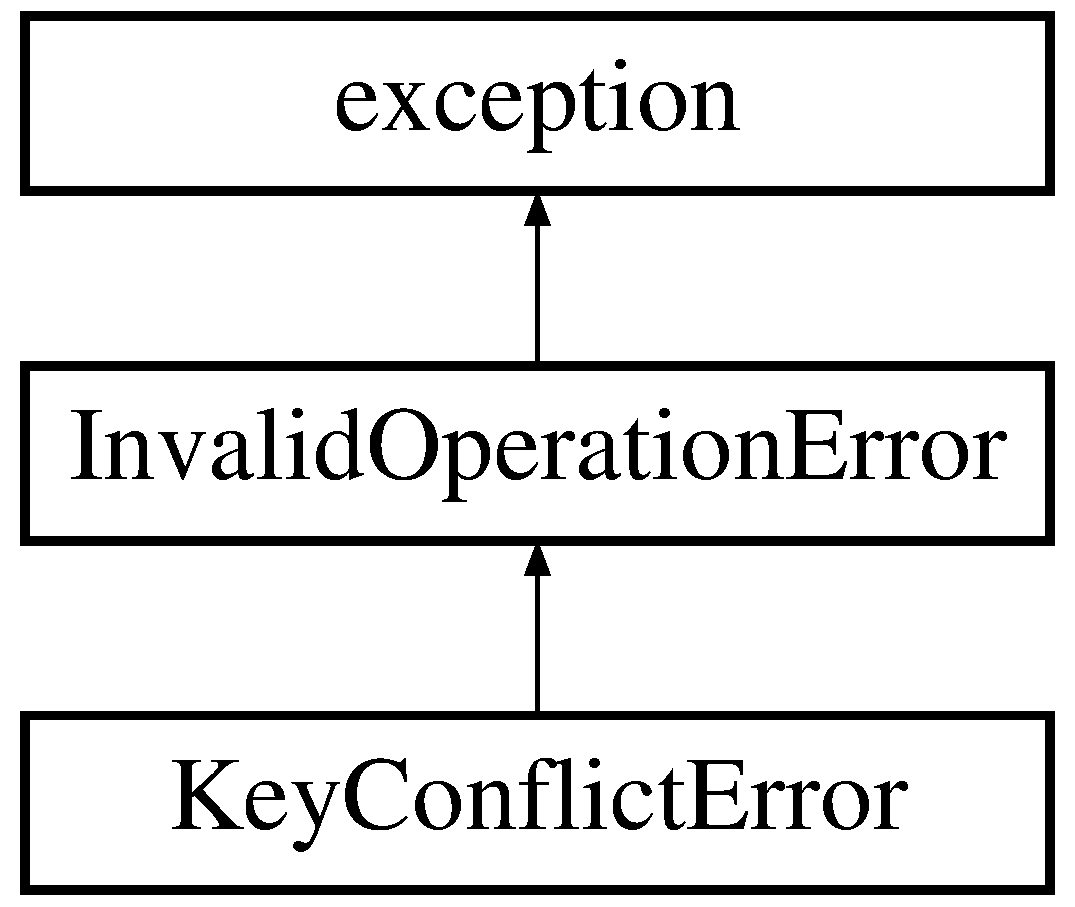
\includegraphics[height=3.000000cm]{class_invalid_operation_error}
\end{center}
\end{figure}
\subsection*{Public Member Functions}
\begin{DoxyCompactItemize}
\item 
\hypertarget{class_invalid_operation_error_a175538ef340664cf364e0310c3c7221d}{{\bfseries Invalid\-Operation\-Error} (const string \&what)}\label{class_invalid_operation_error_a175538ef340664cf364e0310c3c7221d}

\end{DoxyCompactItemize}


The documentation for this class was generated from the following file\-:\begin{DoxyCompactItemize}
\item 
\hyperlink{exception_8h}{exception.\-h}\end{DoxyCompactItemize}

\hypertarget{class_invalid_type_error}{\section{Invalid\-Type\-Error Class Reference}
\label{class_invalid_type_error}\index{Invalid\-Type\-Error@{Invalid\-Type\-Error}}
}


{\ttfamily \#include $<$exception.\-h$>$}

Inheritance diagram for Invalid\-Type\-Error\-:\begin{figure}[H]
\begin{center}
\leavevmode
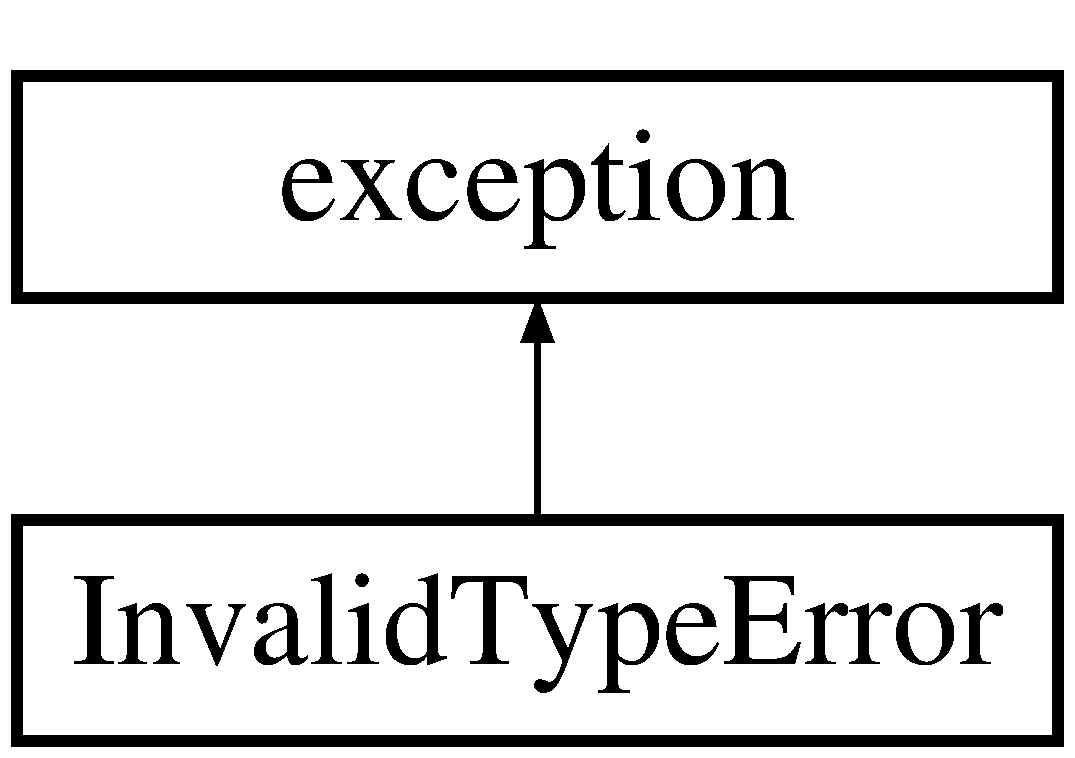
\includegraphics[height=2.000000cm]{class_invalid_type_error}
\end{center}
\end{figure}
\subsection*{Public Member Functions}
\begin{DoxyCompactItemize}
\item 
\hypertarget{class_invalid_type_error_aaa919293fd756aaa32e33dbed1bcaf7b}{{\bfseries Invalid\-Type\-Error} (const string \&what)}\label{class_invalid_type_error_aaa919293fd756aaa32e33dbed1bcaf7b}

\end{DoxyCompactItemize}


\subsection{Detailed Description}
Thrown when the specified value cannot be converted to the requested type. 

The documentation for this class was generated from the following file\-:\begin{DoxyCompactItemize}
\item 
\hyperlink{exception_8h}{exception.\-h}\end{DoxyCompactItemize}

\hypertarget{class_i_o_error}{\section{I\-O\-Error Class Reference}
\label{class_i_o_error}\index{I\-O\-Error@{I\-O\-Error}}
}
Inheritance diagram for I\-O\-Error\-:\begin{figure}[H]
\begin{center}
\leavevmode
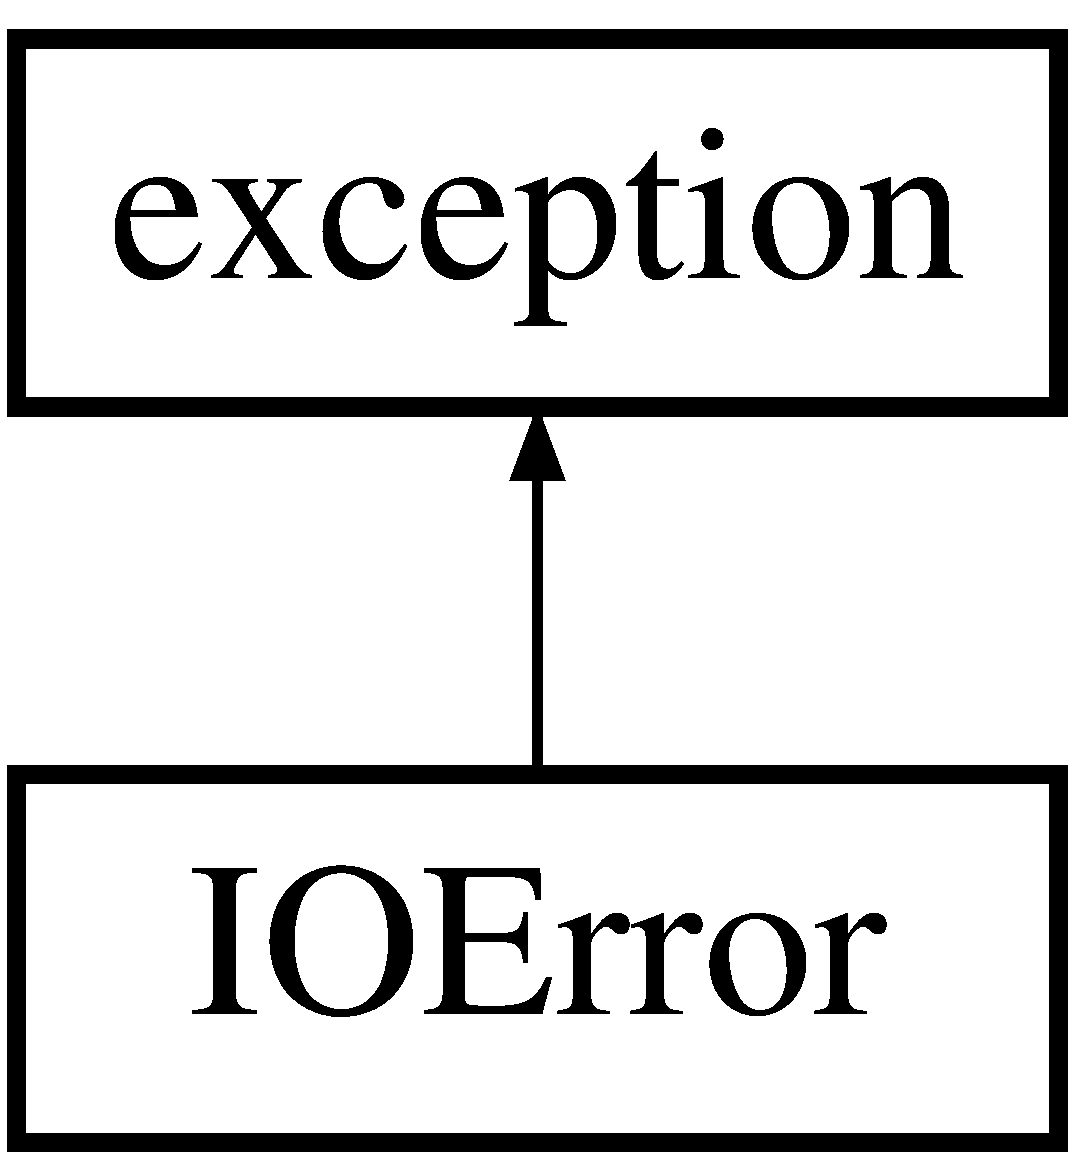
\includegraphics[height=2.000000cm]{class_i_o_error}
\end{center}
\end{figure}
\subsection*{Public Member Functions}
\begin{DoxyCompactItemize}
\item 
\hypertarget{class_i_o_error_aef20e87e03984f98f51706e019a4d141}{{\bfseries I\-O\-Error} (const string \&what)}\label{class_i_o_error_aef20e87e03984f98f51706e019a4d141}

\end{DoxyCompactItemize}


The documentation for this class was generated from the following file\-:\begin{DoxyCompactItemize}
\item 
\hyperlink{exception_8h}{exception.\-h}\end{DoxyCompactItemize}

\hypertarget{class_key_conflict_error}{\section{Key\-Conflict\-Error Class Reference}
\label{class_key_conflict_error}\index{Key\-Conflict\-Error@{Key\-Conflict\-Error}}
}
Inheritance diagram for Key\-Conflict\-Error\-:\begin{figure}[H]
\begin{center}
\leavevmode
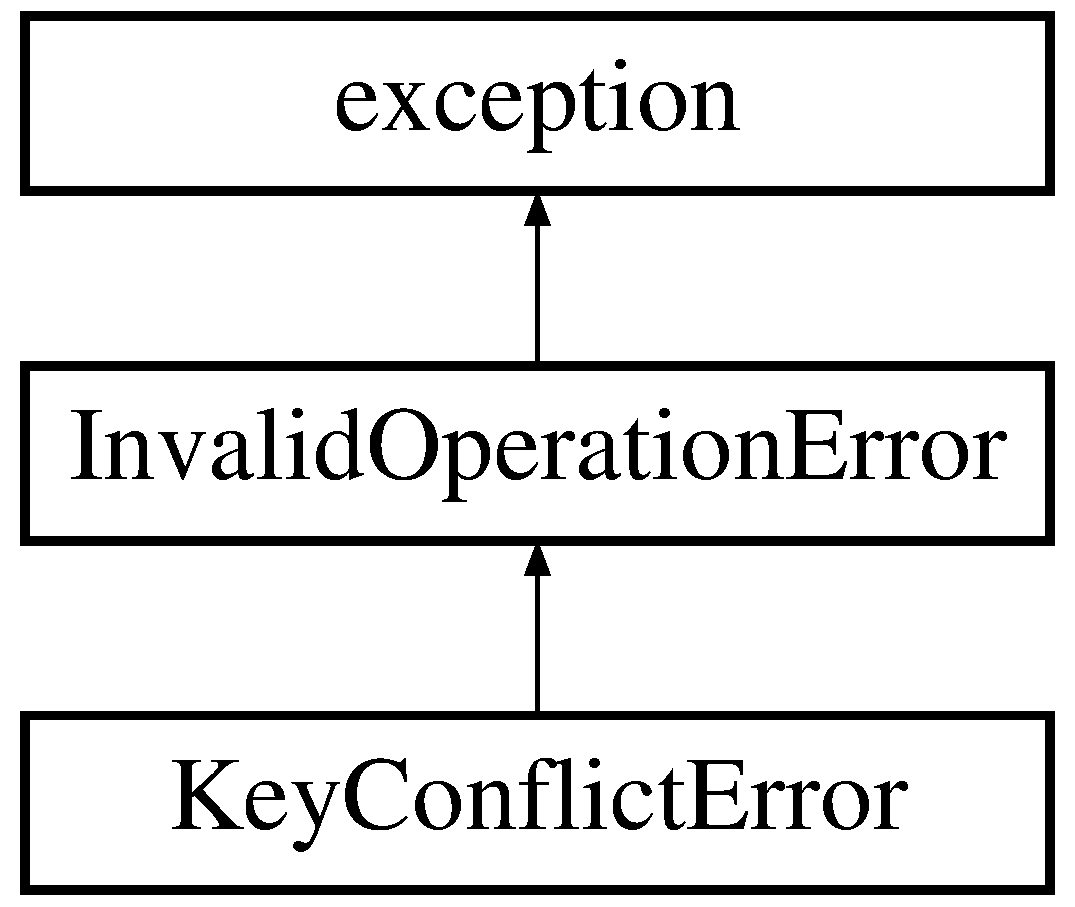
\includegraphics[height=3.000000cm]{class_key_conflict_error}
\end{center}
\end{figure}
\subsection*{Public Member Functions}
\begin{DoxyCompactItemize}
\item 
\hypertarget{class_key_conflict_error_a47c4c27e9542c637d400bf15ef8fb3f4}{{\bfseries Key\-Conflict\-Error} (const string \&what)}\label{class_key_conflict_error_a47c4c27e9542c637d400bf15ef8fb3f4}

\end{DoxyCompactItemize}


The documentation for this class was generated from the following file\-:\begin{DoxyCompactItemize}
\item 
\hyperlink{exception_8h}{exception.\-h}\end{DoxyCompactItemize}

\hypertarget{class_query_syntax_error}{\section{Query\-Syntax\-Error Class Reference}
\label{class_query_syntax_error}\index{Query\-Syntax\-Error@{Query\-Syntax\-Error}}
}
Inheritance diagram for Query\-Syntax\-Error\-:\begin{figure}[H]
\begin{center}
\leavevmode
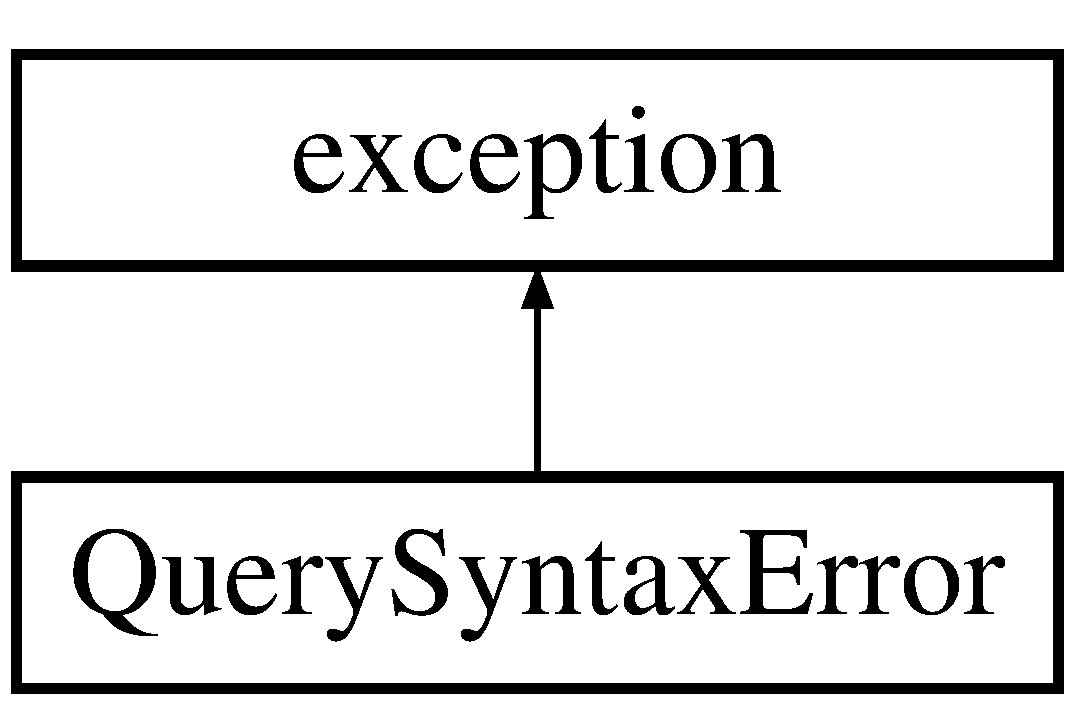
\includegraphics[height=2.000000cm]{class_query_syntax_error}
\end{center}
\end{figure}
\subsection*{Public Member Functions}
\begin{DoxyCompactItemize}
\item 
\hypertarget{class_query_syntax_error_a6259e7507e71776067ee7d36829931d0}{{\bfseries Query\-Syntax\-Error} (const string \&what)}\label{class_query_syntax_error_a6259e7507e71776067ee7d36829931d0}

\end{DoxyCompactItemize}


The documentation for this class was generated from the following file\-:\begin{DoxyCompactItemize}
\item 
\hyperlink{exception_8h}{exception.\-h}\end{DoxyCompactItemize}

\hypertarget{class_record}{\section{Record Class Reference}
\label{class_record}\index{Record@{Record}}
}


{\ttfamily \#include $<$record.\-h$>$}

\subsection*{Public Types}
\begin{DoxyCompactItemize}
\item 
typedef vector$<$ pair$<$ string, \\*
string $>$ $>$\-::const\-\_\-iterator \hyperlink{class_record_ae8a1c90a4d896429d087ccc1f205f9b7}{Record\-Iterator}
\end{DoxyCompactItemize}
\subsection*{Public Member Functions}
\begin{DoxyCompactItemize}
\item 
\hyperlink{class_record_ae8ee53ffec6ff4dac9911517d47e86a5}{Record} ()
\item 
\hyperlink{class_record_af6b85f753bb8dfea3e29728490b3d2a3}{Record} (vector$<$ pair$<$ string, string $>$ $>$ entries)
\item 
\hyperlink{class_record_ae8a1c90a4d896429d087ccc1f205f9b7}{Record\-Iterator} \hyperlink{class_record_a4f65302d712b34e19b8bac9aeff06016}{begin} () const 
\item 
\hyperlink{class_record_ae8a1c90a4d896429d087ccc1f205f9b7}{Record\-Iterator} \hyperlink{class_record_a50ab91b0bb46a381cd3e3b297e4b9d9e}{end} () const 
\item 
{\footnotesize template$<$typename T $>$ }\\T \hyperlink{class_record_a5b6392211018031e67e4d4c599046061}{get} (string field) const 
\item 
{\footnotesize template$<$typename T $>$ }\\void \hyperlink{class_record_ab3efe3a4a4e6a9359bbc82782084c821}{set} (string field, T new\-\_\-value)
\end{DoxyCompactItemize}
\subsection*{Protected Member Functions}
\begin{DoxyCompactItemize}
\item 
\hypertarget{class_record_a851228aba42b5cb2516b29cf6632df8b}{void {\bfseries join} (const \hyperlink{class_record}{Record} \&other)}\label{class_record_a851228aba42b5cb2516b29cf6632df8b}

\item 
\hypertarget{class_record_aba8b5c0a2299a45d068db1ce818051e4}{void {\bfseries erase} (string field)}\label{class_record_aba8b5c0a2299a45d068db1ce818051e4}

\end{DoxyCompactItemize}
\subsection*{Friends}
\begin{DoxyCompactItemize}
\item 
\hypertarget{class_record_af888815e80064bc9fa1035c6265da86e}{class {\bfseries Table}}\label{class_record_af888815e80064bc9fa1035c6265da86e}

\end{DoxyCompactItemize}


\subsection{Detailed Description}
Allows for read and write access of field values.

In the context of a table, fields are known as columns, but within a record they are called fields. 

\subsection{Member Typedef Documentation}
\hypertarget{class_record_ae8a1c90a4d896429d087ccc1f205f9b7}{\index{Record@{Record}!Record\-Iterator@{Record\-Iterator}}
\index{Record\-Iterator@{Record\-Iterator}!Record@{Record}}
\subsubsection[{Record\-Iterator}]{\setlength{\rightskip}{0pt plus 5cm}typedef vector$<$pair$<$string, string$>$ $>$\-::const\-\_\-iterator {\bf Record\-::\-Record\-Iterator}}}\label{class_record_ae8a1c90a4d896429d087ccc1f205f9b7}
A const iterator over the fields in a record.

Each element accessed by the iterator is a pair. The first element is the field name, the second is the value (in string form.) \begin{DoxySeeAlso}{See Also}
\hyperlink{class_record_a4f65302d712b34e19b8bac9aeff06016}{begin()}, \hyperlink{class_record_a50ab91b0bb46a381cd3e3b297e4b9d9e}{end()} 
\end{DoxySeeAlso}


\subsection{Constructor \& Destructor Documentation}
\hypertarget{class_record_ae8ee53ffec6ff4dac9911517d47e86a5}{\index{Record@{Record}!Record@{Record}}
\index{Record@{Record}!Record@{Record}}
\subsubsection[{Record}]{\setlength{\rightskip}{0pt plus 5cm}Record\-::\-Record (
\begin{DoxyParamCaption}
{}
\end{DoxyParamCaption}
)}}\label{class_record_ae8ee53ffec6ff4dac9911517d47e86a5}
Create a record with no fields and no data. \hypertarget{class_record_af6b85f753bb8dfea3e29728490b3d2a3}{\index{Record@{Record}!Record@{Record}}
\index{Record@{Record}!Record@{Record}}
\subsubsection[{Record}]{\setlength{\rightskip}{0pt plus 5cm}Record\-::\-Record (
\begin{DoxyParamCaption}
\item[{vector$<$ pair$<$ string, string $>$ $>$}]{entries}
\end{DoxyParamCaption}
)}}\label{class_record_af6b85f753bb8dfea3e29728490b3d2a3}
Create a record with existing entries 
\begin{DoxyParams}{Parameters}
{\em entries} & a std\-::vector of pairs, with the first element in the pair being the field/column name, and the second element being the value. \\
\hline
\end{DoxyParams}


\subsection{Member Function Documentation}
\hypertarget{class_record_a4f65302d712b34e19b8bac9aeff06016}{\index{Record@{Record}!begin@{begin}}
\index{begin@{begin}!Record@{Record}}
\subsubsection[{begin}]{\setlength{\rightskip}{0pt plus 5cm}{\bf Record\-Iterator} Record\-::begin (
\begin{DoxyParamCaption}
{}
\end{DoxyParamCaption}
) const}}\label{class_record_a4f65302d712b34e19b8bac9aeff06016}
Returns an iterator to the first field in the record.

Note that the Record\-Iterator gives you values in string form. If you want automatic conversions, use {\itshape get} instead.

\begin{DoxySeeAlso}{See Also}
\hyperlink{class_record_a5b6392211018031e67e4d4c599046061}{get()}, \hyperlink{class_record_a50ab91b0bb46a381cd3e3b297e4b9d9e}{end()} 
\end{DoxySeeAlso}
\hypertarget{class_record_a50ab91b0bb46a381cd3e3b297e4b9d9e}{\index{Record@{Record}!end@{end}}
\index{end@{end}!Record@{Record}}
\subsubsection[{end}]{\setlength{\rightskip}{0pt plus 5cm}{\bf Record\-Iterator} Record\-::end (
\begin{DoxyParamCaption}
{}
\end{DoxyParamCaption}
) const}}\label{class_record_a50ab91b0bb46a381cd3e3b297e4b9d9e}
Returns an iterator past the end of the fields in the record. \begin{DoxySeeAlso}{See Also}
\hyperlink{class_record_a4f65302d712b34e19b8bac9aeff06016}{begin()} 
\end{DoxySeeAlso}
\hypertarget{class_record_a5b6392211018031e67e4d4c599046061}{\index{Record@{Record}!get@{get}}
\index{get@{get}!Record@{Record}}
\subsubsection[{get}]{\setlength{\rightskip}{0pt plus 5cm}template$<$typename T $>$ T Record\-::get (
\begin{DoxyParamCaption}
\item[{string}]{field}
\end{DoxyParamCaption}
) const}}\label{class_record_a5b6392211018031e67e4d4c599046061}
Get the value of a field by column name. The field is converted to the requested C++ type if possible (otherwise, an {\itshape \hyperlink{class_invalid_type_error}{Invalid\-Type\-Error}} is thrown.)

Example\-: 
\begin{DoxyCode}
myRecord.get<\textcolor{keywordtype}{int}>(\textcolor{stringliteral}{"age"});
\textcolor{keywordtype}{string} name = myRecord.get<\textcolor{keywordtype}{string}>(\textcolor{stringliteral}{"name"});
\end{DoxyCode}


Throws a {\itshape \hyperlink{class_column_does_not_exist_error}{Column\-Does\-Not\-Exist\-Error}} if {\itshape field} doesn't exist.


\begin{DoxyParams}{Parameters}
{\em T} & The expected type of the field \\
\hline
{\em field} & The name of the field (column) in the record. \\
\hline
\end{DoxyParams}
\hypertarget{class_record_ab3efe3a4a4e6a9359bbc82782084c821}{\index{Record@{Record}!set@{set}}
\index{set@{set}!Record@{Record}}
\subsubsection[{set}]{\setlength{\rightskip}{0pt plus 5cm}template$<$typename T $>$ void Record\-::set (
\begin{DoxyParamCaption}
\item[{string}]{field, }
\item[{T}]{new\-\_\-value}
\end{DoxyParamCaption}
)}}\label{class_record_ab3efe3a4a4e6a9359bbc82782084c821}
Set the value of a field by column name. The field is converted from the given C++ type if possible.

Example\-: 
\begin{DoxyCode}
myRecord.set(\textcolor{stringliteral}{"age"}, 21);
myRecord.set(\textcolor{stringliteral}{"name"}, \textcolor{stringliteral}{"Abraham Lincoln"});
\end{DoxyCode}



\begin{DoxyParams}{Parameters}
{\em T} & The type of {\itshape field}; usually inferred by the compiler. \\
\hline
{\em field} & The name of the field (column) in the record. \\
\hline
\end{DoxyParams}


The documentation for this class was generated from the following file\-:\begin{DoxyCompactItemize}
\item 
record.\-h\end{DoxyCompactItemize}

\hypertarget{class_row_does_not_exist_error}{\section{Row\-Does\-Not\-Exist\-Error Class Reference}
\label{class_row_does_not_exist_error}\index{Row\-Does\-Not\-Exist\-Error@{Row\-Does\-Not\-Exist\-Error}}
}
Inheritance diagram for Row\-Does\-Not\-Exist\-Error\-:\begin{figure}[H]
\begin{center}
\leavevmode
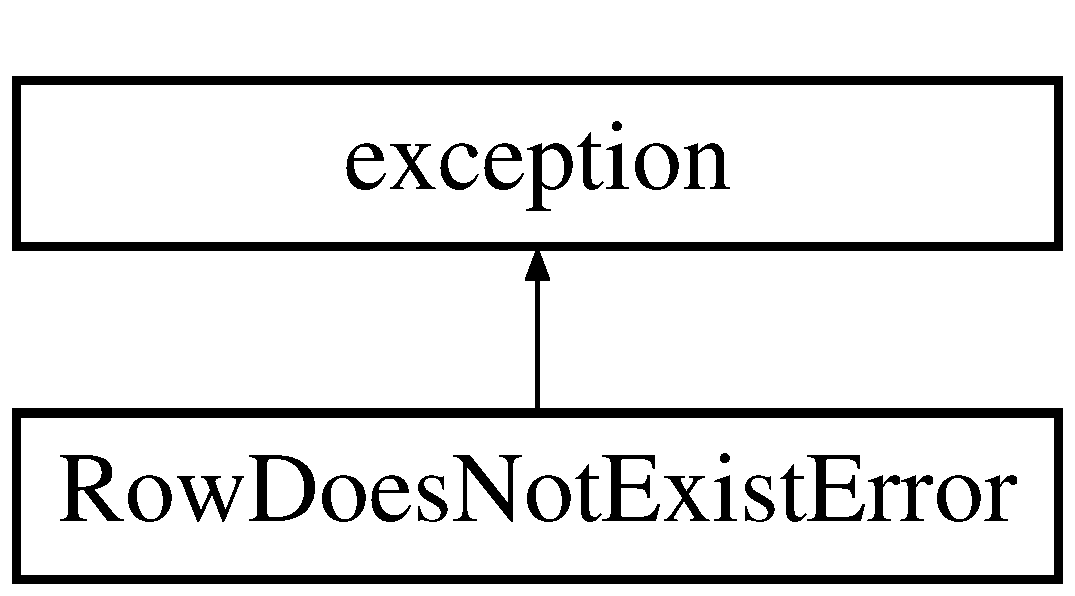
\includegraphics[height=2.000000cm]{class_row_does_not_exist_error}
\end{center}
\end{figure}
\subsection*{Public Member Functions}
\begin{DoxyCompactItemize}
\item 
\hypertarget{class_row_does_not_exist_error_a0b53c63ab8a9220a9a12a44aa3330c36}{{\bfseries Row\-Does\-Not\-Exist\-Error} (const string \&what)}\label{class_row_does_not_exist_error_a0b53c63ab8a9220a9a12a44aa3330c36}

\end{DoxyCompactItemize}


The documentation for this class was generated from the following file\-:\begin{DoxyCompactItemize}
\item 
\hyperlink{exception_8h}{exception.\-h}\end{DoxyCompactItemize}

\hypertarget{class_table}{\section{Table Class Reference}
\label{class_table}\index{Table@{Table}}
}


{\ttfamily \#include $<$table.\-h$>$}

\subsection*{Public Types}
\begin{DoxyCompactItemize}
\item 
enum \hyperlink{class_table_af8f9ec96ecaa35a2e65312b74ddfeae6}{Record\-Type} \{ \\*
\hyperlink{class_table_af8f9ec96ecaa35a2e65312b74ddfeae6a0e9b8fc48315b1aa6736b0a6d1a5dd5c}{undefined\-\_\-type} = 0, 
\hyperlink{class_table_af8f9ec96ecaa35a2e65312b74ddfeae6a0739dd940ab69c758e43e1fd594f8500}{integer} = 1, 
\hyperlink{class_table_af8f9ec96ecaa35a2e65312b74ddfeae6adb56749fe0fd26f3af064ab8b1b695b7}{floating} = 2, 
\hyperlink{class_table_af8f9ec96ecaa35a2e65312b74ddfeae6aa112e11f34f9be73cb2be2b88f193ddb}{varchar} = 3, 
\\*
\hyperlink{class_table_af8f9ec96ecaa35a2e65312b74ddfeae6a31f82673442a5b478c44239c404d921c}{date} = 4, 
\hyperlink{class_table_af8f9ec96ecaa35a2e65312b74ddfeae6ab7605a19d0f66b3e1d92a8270bdbf34b}{time} = 5
 \}
\item 
typedef deque$<$ \hyperlink{class_record}{Record} $>$\\*
\-::const\-\_\-iterator \hyperlink{class_table_aa04536c6711fef7696862b4d94c077e9}{Table\-Iterator}
\item 
\hypertarget{class_table_a15f34139f21ca44eb608b16e5cc8bd75}{typedef vector$<$ pair$<$ string, \\*
\hyperlink{class_table_af8f9ec96ecaa35a2e65312b74ddfeae6}{Record\-Type} $>$ $>$ {\bfseries Column\-List}}\label{class_table_a15f34139f21ca44eb608b16e5cc8bd75}

\end{DoxyCompactItemize}
\subsection*{Public Member Functions}
\begin{DoxyCompactItemize}
\item 
\hyperlink{class_table_a049f2e06391781ae255c6698869c4ad1}{Table} ()
\item 
\hyperlink{class_table_a9d931fcdaa2642148e5bea71dcd824a8}{Table} (const Column\-List \&\hyperlink{class_table_a3185dd0a29eb9fada468a2b42ff9a8a0}{columns})
\item 
\hyperlink{class_table}{Table} $\ast$ \hyperlink{class_table_ae0483f56898b052528eed1ae5391e11d}{clone\-\_\-structure} ()
\item 
void \hyperlink{class_table_a5eda782285dfd05d311de6905dab4e93}{add\-\_\-column} (string column\-\_\-name, \hyperlink{class_table_af8f9ec96ecaa35a2e65312b74ddfeae6}{Record\-Type} type)
\item 
void \hyperlink{class_table_af4c19f81efeece5e7dba4c17d4ee9203}{del\-\_\-column} (string column\-\_\-name)
\item 
void \hyperlink{class_table_ac5c19a55c8527ee267360cd1332317bd}{rename\-\_\-column} (string from, string to)
\item 
Column\-List \hyperlink{class_table_a3185dd0a29eb9fada468a2b42ff9a8a0}{columns} () const 
\item 
unsigned int \hyperlink{class_table_acb9ca5966a6dbae64a4923653031d932}{index\-\_\-for} (string column\-\_\-name) const 
\item 
void \hyperlink{class_table_a38aeaab31fddbd256bc702593a4e8792}{set\-\_\-key} (vector$<$ string $>$ column\-\_\-names)
\item 
vector$<$ string $>$ \hyperlink{class_table_a411f14354a9eb2b85f07fb2187d25271}{key} () const 
\item 
int \hyperlink{class_table_a2c5420361660d9e787487de8d6eb9e44}{size} () const 
\item 
void \hyperlink{class_table_aa1f3a42477818299c83c733e4aa82eb2}{insert} (const \hyperlink{class_record}{Record} \&record)
\item 
\hyperlink{class_table_aa04536c6711fef7696862b4d94c077e9}{Table\-Iterator} \hyperlink{class_table_a020add8ec0eb6fec40695c605adc9038}{begin} () const 
\item 
\hyperlink{class_table_aa04536c6711fef7696862b4d94c077e9}{Table\-Iterator} \hyperlink{class_table_a43c8c8884f3ea7ef66c5de5234e5d93d}{end} () const 
\item 
const \hyperlink{class_record}{Record} \& \hyperlink{class_table_a641c5957ec95abc233450a447c34b820}{first} () const 
\item 
const \hyperlink{class_record}{Record} \& \hyperlink{class_table_afb08a45913f50106dc16388579897134}{last} () const 
\item 
const \hyperlink{class_record}{Record} \& \hyperlink{class_table_a7f27c65febdd226b6973ea082863e0ee}{at} (unsigned int i) const 
\item 
\hyperlink{class_table}{Table} \hyperlink{class_table_a85c83b9f8eeba7cfc7373611297f2194}{cross\-\_\-join} (const \hyperlink{class_table}{Table} \&other) const 
\item 
\hyperlink{class_table}{Table} \hyperlink{class_table_afc179505ae7fdf06d2ec5564a24817dc}{natural\-\_\-join} (const \hyperlink{class_table}{Table} \&other) const 
\item 
int \hyperlink{class_table_a98e0ec7a2a729d9dc5f4de0324e021f5}{count} (string column\-\_\-name) const 
\item 
{\footnotesize template$<$typename T $>$ }\\T \hyperlink{class_table_ab00659a94da98ec7bd60a8a711b2ec77}{sum} (string column\-\_\-name) const 
\item 
{\footnotesize template$<$typename T $>$ }\\T \hyperlink{class_table_a2a4882f99726fba725314e2625ed37ae}{min} (string column\-\_\-name) const 
\item 
{\footnotesize template$<$typename T $>$ }\\T \hyperlink{class_table_abb7aff3403f246965d7557ab592110dd}{max} (string column\-\_\-name) const 
\item 
\hypertarget{class_table_ac6934afdb79cdb140098e0b4fa24acf6}{void {\bfseries drop\-\_\-where} (string where)}\label{class_table_ac6934afdb79cdb140098e0b4fa24acf6}

\item 
\hypertarget{class_table_ad4d6110f8a2d020c4f360cb23554357b}{void {\bfseries update} (string where, string set)}\label{class_table_ad4d6110f8a2d020c4f360cb23554357b}

\end{DoxyCompactItemize}
\subsection*{Static Public Member Functions}
\begin{DoxyCompactItemize}
\item 
\hypertarget{class_table_a9e6d226580485a3eb54ed77dbd09c318}{static bool {\bfseries is\-\_\-valid} (\hyperlink{class_table_af8f9ec96ecaa35a2e65312b74ddfeae6}{Record\-Type} type, string str)}\label{class_table_a9e6d226580485a3eb54ed77dbd09c318}

\end{DoxyCompactItemize}


\subsection{Detailed Description}
A table.

Tables consist of columns (each with a name and a type) and rows (records).

A table may or may not be inside a database. Often it is used for result sets from queries on a larger table. 

\subsection{Member Typedef Documentation}
\hypertarget{class_table_aa04536c6711fef7696862b4d94c077e9}{\index{Table@{Table}!Table\-Iterator@{Table\-Iterator}}
\index{Table\-Iterator@{Table\-Iterator}!Table@{Table}}
\subsubsection[{Table\-Iterator}]{\setlength{\rightskip}{0pt plus 5cm}typedef deque$<${\bf Record}$>$\-::const\-\_\-iterator {\bf Table\-::\-Table\-Iterator}}}\label{class_table_aa04536c6711fef7696862b4d94c077e9}
A const iterator over the records in a table.

Do not depend on the underlying type of Table\-Iterator in your code, but rather a generic iterator interface. 

\subsection{Member Enumeration Documentation}
\hypertarget{class_table_af8f9ec96ecaa35a2e65312b74ddfeae6}{\index{Table@{Table}!Record\-Type@{Record\-Type}}
\index{Record\-Type@{Record\-Type}!Table@{Table}}
\subsubsection[{Record\-Type}]{\setlength{\rightskip}{0pt plus 5cm}enum {\bf Table\-::\-Record\-Type}}}\label{class_table_af8f9ec96ecaa35a2e65312b74ddfeae6}
An enum specifying the type of a column. \begin{Desc}
\item[Enumerator]\par
\begin{description}
\index{undefined\-\_\-type@{undefined\-\_\-type}!Table@{Table}}\index{Table@{Table}!undefined\-\_\-type@{undefined\-\_\-type}}\item[{\em 
\hypertarget{class_table_af8f9ec96ecaa35a2e65312b74ddfeae6a0e9b8fc48315b1aa6736b0a6d1a5dd5c}{undefined\-\_\-type}\label{class_table_af8f9ec96ecaa35a2e65312b74ddfeae6a0e9b8fc48315b1aa6736b0a6d1a5dd5c}
}]Not for normal use. \index{integer@{integer}!Table@{Table}}\index{Table@{Table}!integer@{integer}}\item[{\em 
\hypertarget{class_table_af8f9ec96ecaa35a2e65312b74ddfeae6a0739dd940ab69c758e43e1fd594f8500}{integer}\label{class_table_af8f9ec96ecaa35a2e65312b74ddfeae6a0739dd940ab69c758e43e1fd594f8500}
}]32-\/bit signed integer \index{floating@{floating}!Table@{Table}}\index{Table@{Table}!floating@{floating}}\item[{\em 
\hypertarget{class_table_af8f9ec96ecaa35a2e65312b74ddfeae6adb56749fe0fd26f3af064ab8b1b695b7}{floating}\label{class_table_af8f9ec96ecaa35a2e65312b74ddfeae6adb56749fe0fd26f3af064ab8b1b695b7}
}]32-\/bit floating point \index{varchar@{varchar}!Table@{Table}}\index{Table@{Table}!varchar@{varchar}}\item[{\em 
\hypertarget{class_table_af8f9ec96ecaa35a2e65312b74ddfeae6aa112e11f34f9be73cb2be2b88f193ddb}{varchar}\label{class_table_af8f9ec96ecaa35a2e65312b74ddfeae6aa112e11f34f9be73cb2be2b88f193ddb}
}]Variable-\/length string. \index{date@{date}!Table@{Table}}\index{Table@{Table}!date@{date}}\item[{\em 
\hypertarget{class_table_af8f9ec96ecaa35a2e65312b74ddfeae6a31f82673442a5b478c44239c404d921c}{date}\label{class_table_af8f9ec96ecaa35a2e65312b74ddfeae6a31f82673442a5b478c44239c404d921c}
}]Date with no time. \index{time@{time}!Table@{Table}}\index{Table@{Table}!time@{time}}\item[{\em 
\hypertarget{class_table_af8f9ec96ecaa35a2e65312b74ddfeae6ab7605a19d0f66b3e1d92a8270bdbf34b}{time}\label{class_table_af8f9ec96ecaa35a2e65312b74ddfeae6ab7605a19d0f66b3e1d92a8270bdbf34b}
}]Time without time zone. \end{description}
\end{Desc}


\subsection{Constructor \& Destructor Documentation}
\hypertarget{class_table_a049f2e06391781ae255c6698869c4ad1}{\index{Table@{Table}!Table@{Table}}
\index{Table@{Table}!Table@{Table}}
\subsubsection[{Table}]{\setlength{\rightskip}{0pt plus 5cm}Table\-::\-Table (
\begin{DoxyParamCaption}
{}
\end{DoxyParamCaption}
)}}\label{class_table_a049f2e06391781ae255c6698869c4ad1}
Creates a table with no rows or columns. \hypertarget{class_table_a9d931fcdaa2642148e5bea71dcd824a8}{\index{Table@{Table}!Table@{Table}}
\index{Table@{Table}!Table@{Table}}
\subsubsection[{Table}]{\setlength{\rightskip}{0pt plus 5cm}Table\-::\-Table (
\begin{DoxyParamCaption}
\item[{const Column\-List \&}]{columns}
\end{DoxyParamCaption}
)}}\label{class_table_a9d931fcdaa2642148e5bea71dcd824a8}
Creates a table with the given column names and types and no rows.

Example\-: 
\begin{DoxyCode}
Table::ColumnList \hyperlink{class_table_a3185dd0a29eb9fada468a2b42ff9a8a0}{columns};
columns.push\_back(make\_pair(\textcolor{stringliteral}{"id"}, \hyperlink{class_table_af8f9ec96ecaa35a2e65312b74ddfeae6a0739dd940ab69c758e43e1fd594f8500}{Table::integer}));
columns.push\_back(make\_pair(\textcolor{stringliteral}{"name"}, \hyperlink{class_table_af8f9ec96ecaa35a2e65312b74ddfeae6aa112e11f34f9be73cb2be2b88f193ddb}{Table::varchar}));
\hyperlink{class_table}{Table} my\_table(columns);
\end{DoxyCode}
 

\subsection{Member Function Documentation}
\hypertarget{class_table_a5eda782285dfd05d311de6905dab4e93}{\index{Table@{Table}!add\-\_\-column@{add\-\_\-column}}
\index{add\-\_\-column@{add\-\_\-column}!Table@{Table}}
\subsubsection[{add\-\_\-column}]{\setlength{\rightskip}{0pt plus 5cm}void Table\-::add\-\_\-column (
\begin{DoxyParamCaption}
\item[{string}]{column\-\_\-name, }
\item[{{\bf Record\-Type}}]{type}
\end{DoxyParamCaption}
)}}\label{class_table_a5eda782285dfd05d311de6905dab4e93}
Adds a column to the end of the table.

Existing entries will be N\-U\-L\-L for this column. \hypertarget{class_table_a7f27c65febdd226b6973ea082863e0ee}{\index{Table@{Table}!at@{at}}
\index{at@{at}!Table@{Table}}
\subsubsection[{at}]{\setlength{\rightskip}{0pt plus 5cm}const {\bf Record}\& Table\-::at (
\begin{DoxyParamCaption}
\item[{unsigned int}]{i}
\end{DoxyParamCaption}
) const}}\label{class_table_a7f27c65febdd226b6973ea082863e0ee}
Returns the $\ast$i$\ast$th record in the table, starting at 0. Throws a {\itshape \hyperlink{class_row_does_not_exist_error}{Row\-Does\-Not\-Exist\-Error}} if {\itshape i} is out of range ($<$ 0 or $>$= \hyperlink{class_table_a2c5420361660d9e787487de8d6eb9e44}{size()}.) \begin{DoxySeeAlso}{See Also}
\hyperlink{class_table_a641c5957ec95abc233450a447c34b820}{first()}, \hyperlink{class_table_afb08a45913f50106dc16388579897134}{last()}, \hyperlink{class_table_a020add8ec0eb6fec40695c605adc9038}{begin()}, \hyperlink{class_table_a43c8c8884f3ea7ef66c5de5234e5d93d}{end()} 
\end{DoxySeeAlso}
\hypertarget{class_table_a020add8ec0eb6fec40695c605adc9038}{\index{Table@{Table}!begin@{begin}}
\index{begin@{begin}!Table@{Table}}
\subsubsection[{begin}]{\setlength{\rightskip}{0pt plus 5cm}{\bf Table\-Iterator} Table\-::begin (
\begin{DoxyParamCaption}
{}
\end{DoxyParamCaption}
) const}}\label{class_table_a020add8ec0eb6fec40695c605adc9038}
Returns an iterator to the first record in the table.

A \hyperlink{class_table}{Table} can be treated as a container. The {\itshape begin} and {\itshape end} functions correspond to C++ S\-T\-L container begin and end functions, as do {\itshape first}, {\itshape last}, and {\itshape at}.

\begin{DoxySeeAlso}{See Also}
\hyperlink{class_table_a43c8c8884f3ea7ef66c5de5234e5d93d}{end()}, \hyperlink{class_table_a641c5957ec95abc233450a447c34b820}{first()}, \hyperlink{class_table_afb08a45913f50106dc16388579897134}{last()}, \hyperlink{class_table_a7f27c65febdd226b6973ea082863e0ee}{at()} 
\end{DoxySeeAlso}
\hypertarget{class_table_ae0483f56898b052528eed1ae5391e11d}{\index{Table@{Table}!clone\-\_\-structure@{clone\-\_\-structure}}
\index{clone\-\_\-structure@{clone\-\_\-structure}!Table@{Table}}
\subsubsection[{clone\-\_\-structure}]{\setlength{\rightskip}{0pt plus 5cm}{\bf Table}$\ast$ Table\-::clone\-\_\-structure (
\begin{DoxyParamCaption}
{}
\end{DoxyParamCaption}
)}}\label{class_table_ae0483f56898b052528eed1ae5391e11d}
Returns a pointer to a new table with the same columns and keys \hypertarget{class_table_a3185dd0a29eb9fada468a2b42ff9a8a0}{\index{Table@{Table}!columns@{columns}}
\index{columns@{columns}!Table@{Table}}
\subsubsection[{columns}]{\setlength{\rightskip}{0pt plus 5cm}Column\-List Table\-::columns (
\begin{DoxyParamCaption}
{}
\end{DoxyParamCaption}
) const}}\label{class_table_a3185dd0a29eb9fada468a2b42ff9a8a0}
Returns a list of columns and their types. \hypertarget{class_table_a98e0ec7a2a729d9dc5f4de0324e021f5}{\index{Table@{Table}!count@{count}}
\index{count@{count}!Table@{Table}}
\subsubsection[{count}]{\setlength{\rightskip}{0pt plus 5cm}int Table\-::count (
\begin{DoxyParamCaption}
\item[{string}]{column\-\_\-name}
\end{DoxyParamCaption}
) const}}\label{class_table_a98e0ec7a2a729d9dc5f4de0324e021f5}
Computes the number of non-\/\-N\-U\-L\-L values in the given column in the table. Throws a {\itshape \hyperlink{class_column_does_not_exist_error}{Column\-Does\-Not\-Exist\-Error}} if {\itshape column\-\_\-name} doesn't exist. \hypertarget{class_table_a85c83b9f8eeba7cfc7373611297f2194}{\index{Table@{Table}!cross\-\_\-join@{cross\-\_\-join}}
\index{cross\-\_\-join@{cross\-\_\-join}!Table@{Table}}
\subsubsection[{cross\-\_\-join}]{\setlength{\rightskip}{0pt plus 5cm}{\bf Table} Table\-::cross\-\_\-join (
\begin{DoxyParamCaption}
\item[{const {\bf Table} \&}]{other}
\end{DoxyParamCaption}
) const}}\label{class_table_a85c83b9f8eeba7cfc7373611297f2194}
Computes a cross join with another table.

A cross join contains every possible combination of rows in the two tables. \hypertarget{class_table_af4c19f81efeece5e7dba4c17d4ee9203}{\index{Table@{Table}!del\-\_\-column@{del\-\_\-column}}
\index{del\-\_\-column@{del\-\_\-column}!Table@{Table}}
\subsubsection[{del\-\_\-column}]{\setlength{\rightskip}{0pt plus 5cm}void Table\-::del\-\_\-column (
\begin{DoxyParamCaption}
\item[{string}]{column\-\_\-name}
\end{DoxyParamCaption}
)}}\label{class_table_af4c19f81efeece5e7dba4c17d4ee9203}
Deletes a column, erasing any associated data.

Throws a {\itshape \hyperlink{class_column_does_not_exist_error}{Column\-Does\-Not\-Exist\-Error}} if {\itshape column\-\_\-name} doesn't exist. \hypertarget{class_table_a43c8c8884f3ea7ef66c5de5234e5d93d}{\index{Table@{Table}!end@{end}}
\index{end@{end}!Table@{Table}}
\subsubsection[{end}]{\setlength{\rightskip}{0pt plus 5cm}{\bf Table\-Iterator} Table\-::end (
\begin{DoxyParamCaption}
{}
\end{DoxyParamCaption}
) const}}\label{class_table_a43c8c8884f3ea7ef66c5de5234e5d93d}
Returns an iterator past the end of the last record in the table. \begin{DoxySeeAlso}{See Also}
\hyperlink{class_table_a020add8ec0eb6fec40695c605adc9038}{begin()} 
\end{DoxySeeAlso}
\hypertarget{class_table_a641c5957ec95abc233450a447c34b820}{\index{Table@{Table}!first@{first}}
\index{first@{first}!Table@{Table}}
\subsubsection[{first}]{\setlength{\rightskip}{0pt plus 5cm}const {\bf Record}\& Table\-::first (
\begin{DoxyParamCaption}
{}
\end{DoxyParamCaption}
) const}}\label{class_table_a641c5957ec95abc233450a447c34b820}
Returns the first record in the table. \begin{DoxySeeAlso}{See Also}
\hyperlink{class_table_afb08a45913f50106dc16388579897134}{last()}, \hyperlink{class_table_a7f27c65febdd226b6973ea082863e0ee}{at()} 
\end{DoxySeeAlso}
\hypertarget{class_table_acb9ca5966a6dbae64a4923653031d932}{\index{Table@{Table}!index\-\_\-for@{index\-\_\-for}}
\index{index\-\_\-for@{index\-\_\-for}!Table@{Table}}
\subsubsection[{index\-\_\-for}]{\setlength{\rightskip}{0pt plus 5cm}unsigned int Table\-::index\-\_\-for (
\begin{DoxyParamCaption}
\item[{string}]{column\-\_\-name}
\end{DoxyParamCaption}
) const}}\label{class_table_acb9ca5966a6dbae64a4923653031d932}
Returns the index of the column specified in column\-\_\-name, i.\-e. for accessing records. Throws a {\itshape \hyperlink{class_column_does_not_exist_error}{Column\-Does\-Not\-Exist\-Error}} if {\itshape from} doesn't exist. \hypertarget{class_table_aa1f3a42477818299c83c733e4aa82eb2}{\index{Table@{Table}!insert@{insert}}
\index{insert@{insert}!Table@{Table}}
\subsubsection[{insert}]{\setlength{\rightskip}{0pt plus 5cm}void Table\-::insert (
\begin{DoxyParamCaption}
\item[{const {\bf Record} \&}]{record}
\end{DoxyParamCaption}
)}}\label{class_table_aa1f3a42477818299c83c733e4aa82eb2}
Inserts a row at the end of the table. Throws a {\itshape \hyperlink{class_key_conflict_error}{Key\-Conflict\-Error}} if this record would cause a primary key conflict. \hypertarget{class_table_a411f14354a9eb2b85f07fb2187d25271}{\index{Table@{Table}!key@{key}}
\index{key@{key}!Table@{Table}}
\subsubsection[{key}]{\setlength{\rightskip}{0pt plus 5cm}vector$<$string$>$ Table\-::key (
\begin{DoxyParamCaption}
{}
\end{DoxyParamCaption}
) const}}\label{class_table_a411f14354a9eb2b85f07fb2187d25271}
Returns the column names that make up the key for this table.

If there is no key, returns an empty vector. \hypertarget{class_table_afb08a45913f50106dc16388579897134}{\index{Table@{Table}!last@{last}}
\index{last@{last}!Table@{Table}}
\subsubsection[{last}]{\setlength{\rightskip}{0pt plus 5cm}const {\bf Record}\& Table\-::last (
\begin{DoxyParamCaption}
{}
\end{DoxyParamCaption}
) const}}\label{class_table_afb08a45913f50106dc16388579897134}
Returns the last record in the table. \begin{DoxySeeAlso}{See Also}
\hyperlink{class_table_a641c5957ec95abc233450a447c34b820}{first()}, \hyperlink{class_table_a7f27c65febdd226b6973ea082863e0ee}{at()} 
\end{DoxySeeAlso}
\hypertarget{class_table_abb7aff3403f246965d7557ab592110dd}{\index{Table@{Table}!max@{max}}
\index{max@{max}!Table@{Table}}
\subsubsection[{max}]{\setlength{\rightskip}{0pt plus 5cm}template$<$typename T $>$ T Table\-::max (
\begin{DoxyParamCaption}
\item[{string}]{column\-\_\-name}
\end{DoxyParamCaption}
) const}}\label{class_table_abb7aff3403f246965d7557ab592110dd}
Computes the largest value of all values in the given column in the table. Works for all column types.

Throws a {\itshape \hyperlink{class_column_does_not_exist_error}{Column\-Does\-Not\-Exist\-Error}} if {\itshape column\-\_\-name} doesn't exist. Throws an {\itshape \hyperlink{class_invalid_type_error}{Invalid\-Type\-Error}} if the column cannot be converted to type T. \hypertarget{class_table_a2a4882f99726fba725314e2625ed37ae}{\index{Table@{Table}!min@{min}}
\index{min@{min}!Table@{Table}}
\subsubsection[{min}]{\setlength{\rightskip}{0pt plus 5cm}template$<$typename T $>$ T Table\-::min (
\begin{DoxyParamCaption}
\item[{string}]{column\-\_\-name}
\end{DoxyParamCaption}
) const}}\label{class_table_a2a4882f99726fba725314e2625ed37ae}
Computes the smallest value of all values in the given column in the table. Works for all column types.

Throws a {\itshape \hyperlink{class_column_does_not_exist_error}{Column\-Does\-Not\-Exist\-Error}} if {\itshape column\-\_\-name} doesn't exist. Throws an {\itshape \hyperlink{class_invalid_type_error}{Invalid\-Type\-Error}} if the column cannot be converted to type T. \hypertarget{class_table_afc179505ae7fdf06d2ec5564a24817dc}{\index{Table@{Table}!natural\-\_\-join@{natural\-\_\-join}}
\index{natural\-\_\-join@{natural\-\_\-join}!Table@{Table}}
\subsubsection[{natural\-\_\-join}]{\setlength{\rightskip}{0pt plus 5cm}{\bf Table} Table\-::natural\-\_\-join (
\begin{DoxyParamCaption}
\item[{const {\bf Table} \&}]{other}
\end{DoxyParamCaption}
) const}}\label{class_table_afc179505ae7fdf06d2ec5564a24817dc}
Computes a natural join with another table.

The other table should have a key, and this table should have columns matching that key.

Throws an {\itshape \hyperlink{class_invalid_operation_error}{Invalid\-Operation\-Error}} if the above conditions are not met. \hypertarget{class_table_ac5c19a55c8527ee267360cd1332317bd}{\index{Table@{Table}!rename\-\_\-column@{rename\-\_\-column}}
\index{rename\-\_\-column@{rename\-\_\-column}!Table@{Table}}
\subsubsection[{rename\-\_\-column}]{\setlength{\rightskip}{0pt plus 5cm}void Table\-::rename\-\_\-column (
\begin{DoxyParamCaption}
\item[{string}]{from, }
\item[{string}]{to}
\end{DoxyParamCaption}
)}}\label{class_table_ac5c19a55c8527ee267360cd1332317bd}
Renames a column, keeping the existing type and data. Throws a {\itshape \hyperlink{class_column_does_not_exist_error}{Column\-Does\-Not\-Exist\-Error}} if {\itshape from} doesn't exist. \hypertarget{class_table_a38aeaab31fddbd256bc702593a4e8792}{\index{Table@{Table}!set\-\_\-key@{set\-\_\-key}}
\index{set\-\_\-key@{set\-\_\-key}!Table@{Table}}
\subsubsection[{set\-\_\-key}]{\setlength{\rightskip}{0pt plus 5cm}void Table\-::set\-\_\-key (
\begin{DoxyParamCaption}
\item[{vector$<$ string $>$}]{column\-\_\-names}
\end{DoxyParamCaption}
)}}\label{class_table_a38aeaab31fddbd256bc702593a4e8792}
Defines the tuple of columns used as a key. This function must be called before inserting any rows into the table.


\begin{DoxyParams}{Parameters}
{\em columns} & A list of column names that make up the key.\\
\hline
\end{DoxyParams}
Every row in the table must have a unique key. If a new row is inserted with a key that already exists in the table, insertion will fail.

Throws a {\itshape \hyperlink{class_column_does_not_exist_error}{Column\-Does\-Not\-Exist\-Error}} if any of the {\itshape column\-\_\-names} don't exist. Throws an {\itshape \hyperlink{class_invalid_operation_error}{Invalid\-Operation\-Error}} if called on a table with rows. \hypertarget{class_table_a2c5420361660d9e787487de8d6eb9e44}{\index{Table@{Table}!size@{size}}
\index{size@{size}!Table@{Table}}
\subsubsection[{size}]{\setlength{\rightskip}{0pt plus 5cm}int Table\-::size (
\begin{DoxyParamCaption}
{}
\end{DoxyParamCaption}
) const}}\label{class_table_a2c5420361660d9e787487de8d6eb9e44}
Returns the number of rows in the table. \hypertarget{class_table_ab00659a94da98ec7bd60a8a711b2ec77}{\index{Table@{Table}!sum@{sum}}
\index{sum@{sum}!Table@{Table}}
\subsubsection[{sum}]{\setlength{\rightskip}{0pt plus 5cm}template$<$typename T $>$ T Table\-::sum (
\begin{DoxyParamCaption}
\item[{string}]{column\-\_\-name}
\end{DoxyParamCaption}
) const}}\label{class_table_ab00659a94da98ec7bd60a8a711b2ec77}
Computes the sum of all values in the given column in the table. Works for numeric column types only.

Throws a {\itshape \hyperlink{class_column_does_not_exist_error}{Column\-Does\-Not\-Exist\-Error}} if {\itshape column\-\_\-name} doesn't exist. Throws an {\itshape \hyperlink{class_invalid_operation_error}{Invalid\-Operation\-Error}} if the column is not numeric. 

The documentation for this class was generated from the following file\-:\begin{DoxyCompactItemize}
\item 
table.\-h\end{DoxyCompactItemize}

\hypertarget{class_table_does_not_exist_error}{\section{Table\-Does\-Not\-Exist\-Error Class Reference}
\label{class_table_does_not_exist_error}\index{Table\-Does\-Not\-Exist\-Error@{Table\-Does\-Not\-Exist\-Error}}
}
Inheritance diagram for Table\-Does\-Not\-Exist\-Error\-:\begin{figure}[H]
\begin{center}
\leavevmode
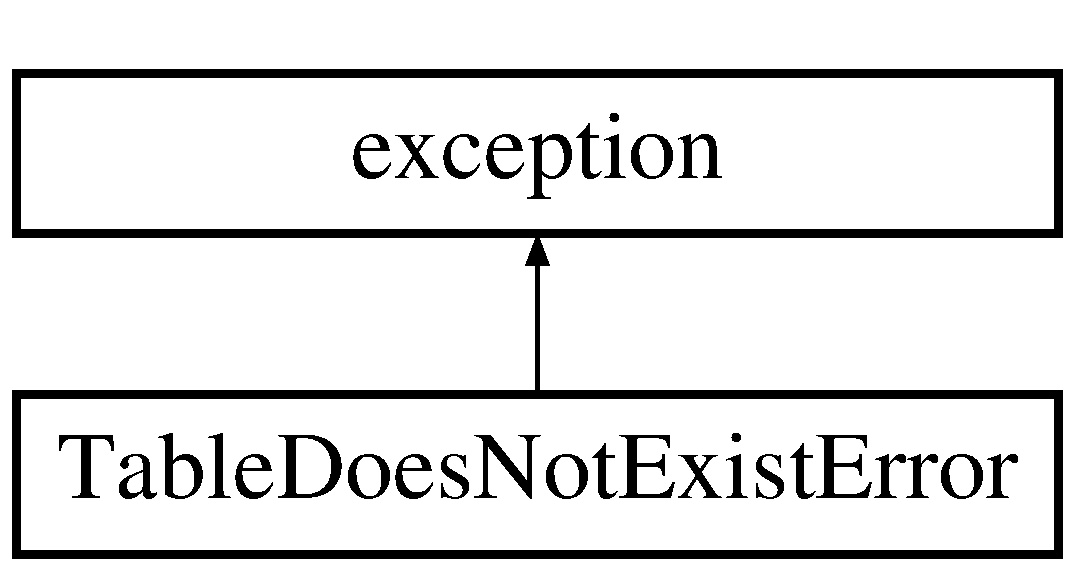
\includegraphics[height=2.000000cm]{class_table_does_not_exist_error}
\end{center}
\end{figure}
\subsection*{Public Member Functions}
\begin{DoxyCompactItemize}
\item 
\hypertarget{class_table_does_not_exist_error_a2e350ef61eb9d5fc3449cbc04155aad7}{{\bfseries Table\-Does\-Not\-Exist\-Error} (const string \&what)}\label{class_table_does_not_exist_error_a2e350ef61eb9d5fc3449cbc04155aad7}

\end{DoxyCompactItemize}


The documentation for this class was generated from the following file\-:\begin{DoxyCompactItemize}
\item 
\hyperlink{exception_8h}{exception.\-h}\end{DoxyCompactItemize}

\hypertarget{struct_type_is_valid}{\section{Type\-Is\-Valid$<$ T $>$ Struct Template Reference}
\label{struct_type_is_valid}\index{Type\-Is\-Valid$<$ T $>$@{Type\-Is\-Valid$<$ T $>$}}
}
\subsection*{Static Public Attributes}
\begin{DoxyCompactItemize}
\item 
\hypertarget{struct_type_is_valid_aaebef75098d48be14ff63ee9fd15a58a}{static const bool {\bfseries value} = false}\label{struct_type_is_valid_aaebef75098d48be14ff63ee9fd15a58a}

\end{DoxyCompactItemize}


The documentation for this struct was generated from the following file\-:\begin{DoxyCompactItemize}
\item 
record.\-h\end{DoxyCompactItemize}

\hypertarget{struct_type_is_valid_3_01const_01char_01_5_01_4}{\section{Type\-Is\-Valid$<$ const char $\ast$ $>$ Struct Template Reference}
\label{struct_type_is_valid_3_01const_01char_01_5_01_4}\index{Type\-Is\-Valid$<$ const char $\ast$ $>$@{Type\-Is\-Valid$<$ const char $\ast$ $>$}}
}
\subsection*{Static Public Attributes}
\begin{DoxyCompactItemize}
\item 
\hypertarget{struct_type_is_valid_3_01const_01char_01_5_01_4_a223f69dcbfa69c7a5c0005bafdc538fb}{static const bool {\bfseries value} = true}\label{struct_type_is_valid_3_01const_01char_01_5_01_4_a223f69dcbfa69c7a5c0005bafdc538fb}

\end{DoxyCompactItemize}


The documentation for this struct was generated from the following file\-:\begin{DoxyCompactItemize}
\item 
record.\-h\end{DoxyCompactItemize}

\hypertarget{struct_type_is_valid_3_01double_01_4}{\section{Type\-Is\-Valid$<$ double $>$ Struct Template Reference}
\label{struct_type_is_valid_3_01double_01_4}\index{Type\-Is\-Valid$<$ double $>$@{Type\-Is\-Valid$<$ double $>$}}
}
\subsection*{Static Public Attributes}
\begin{DoxyCompactItemize}
\item 
\hypertarget{struct_type_is_valid_3_01double_01_4_a50347ed03137ab28704f0331b1d6602c}{static const bool {\bfseries value} = true}\label{struct_type_is_valid_3_01double_01_4_a50347ed03137ab28704f0331b1d6602c}

\end{DoxyCompactItemize}


The documentation for this struct was generated from the following file\-:\begin{DoxyCompactItemize}
\item 
record.\-h\end{DoxyCompactItemize}

\hypertarget{struct_type_is_valid_3_01float_01_4}{\section{Type\-Is\-Valid$<$ float $>$ Struct Template Reference}
\label{struct_type_is_valid_3_01float_01_4}\index{Type\-Is\-Valid$<$ float $>$@{Type\-Is\-Valid$<$ float $>$}}
}
\subsection*{Static Public Attributes}
\begin{DoxyCompactItemize}
\item 
\hypertarget{struct_type_is_valid_3_01float_01_4_abc00b5d96ff8334ffeda51c0c9eb0c50}{static const bool {\bfseries value} = true}\label{struct_type_is_valid_3_01float_01_4_abc00b5d96ff8334ffeda51c0c9eb0c50}

\end{DoxyCompactItemize}


The documentation for this struct was generated from the following file\-:\begin{DoxyCompactItemize}
\item 
record.\-h\end{DoxyCompactItemize}

\hypertarget{struct_type_is_valid_3_01int_01_4}{\section{Type\-Is\-Valid$<$ int $>$ Struct Template Reference}
\label{struct_type_is_valid_3_01int_01_4}\index{Type\-Is\-Valid$<$ int $>$@{Type\-Is\-Valid$<$ int $>$}}
}
\subsection*{Static Public Attributes}
\begin{DoxyCompactItemize}
\item 
\hypertarget{struct_type_is_valid_3_01int_01_4_a72938ec96190ff98ef01c1403e6fe8e8}{static const bool {\bfseries value} = true}\label{struct_type_is_valid_3_01int_01_4_a72938ec96190ff98ef01c1403e6fe8e8}

\end{DoxyCompactItemize}


The documentation for this struct was generated from the following file\-:\begin{DoxyCompactItemize}
\item 
record.\-h\end{DoxyCompactItemize}

\hypertarget{struct_type_is_valid_3_01string_01_4}{\section{Type\-Is\-Valid$<$ string $>$ Struct Template Reference}
\label{struct_type_is_valid_3_01string_01_4}\index{Type\-Is\-Valid$<$ string $>$@{Type\-Is\-Valid$<$ string $>$}}
}
\subsection*{Static Public Attributes}
\begin{DoxyCompactItemize}
\item 
\hypertarget{struct_type_is_valid_3_01string_01_4_a8313dbae58c48e7b4e81e8fee5af320c}{static const bool {\bfseries value} = true}\label{struct_type_is_valid_3_01string_01_4_a8313dbae58c48e7b4e81e8fee5af320c}

\end{DoxyCompactItemize}


The documentation for this struct was generated from the following file\-:\begin{DoxyCompactItemize}
\item 
record.\-h\end{DoxyCompactItemize}

\chapter{File Documentation}
\hypertarget{exception_8h}{\section{exception.\-h File Reference}
\label{exception_8h}\index{exception.\-h@{exception.\-h}}
}
{\ttfamily \#include $<$stdexcept$>$}\\*
\subsection*{Classes}
\begin{DoxyCompactItemize}
\item 
class \hyperlink{class_column_does_not_exist_error}{Column\-Does\-Not\-Exist\-Error}
\item 
class \hyperlink{class_row_does_not_exist_error}{Row\-Does\-Not\-Exist\-Error}
\item 
class \hyperlink{class_table_does_not_exist_error}{Table\-Does\-Not\-Exist\-Error}
\item 
class \hyperlink{class_invalid_operation_error}{Invalid\-Operation\-Error}
\item 
class \hyperlink{class_key_conflict_error}{Key\-Conflict\-Error}
\item 
class \hyperlink{class_invalid_type_error}{Invalid\-Type\-Error}
\item 
class \hyperlink{class_query_syntax_error}{Query\-Syntax\-Error}
\item 
class \hyperlink{class_i_o_error}{I\-O\-Error}
\end{DoxyCompactItemize}
\subsection*{Macros}
\begin{DoxyCompactItemize}
\item 
\hypertarget{exception_8h_a3472d8cdbb788d5f1815b3522595bc49}{\#define {\bfseries E\-X\-P\-O\-R\-T}~\-\_\-\-\_\-declspec(dllexport)}\label{exception_8h_a3472d8cdbb788d5f1815b3522595bc49}

\end{DoxyCompactItemize}


\subsection{Detailed Description}
Defines the exception classes used by this database.

Every exception inherits from std\-::exception, and a detailed message can be obtained using {\itshape what()}. 
\addcontentsline{toc}{part}{Index}
\printindex
\end{document}
